\documentclass[letterpaper,12pt]{article}
\usepackage{tabularx} % extra features for tabular environment
\usepackage{tikz}
\usetikzlibrary{matrix,calc}
\usepackage{caption}
\usepackage{subfigure}
\usepackage{amsmath}  % improve math presentation
\usepackage{graphicx} % takes care of graphic including machinery
\usepackage[margin=1in,letterpaper]{geometry} % decreases margins
\usepackage{cite} % takes care of citations
\usepackage[final]{hyperref} % adds hyper links inside the generated pdf file
\hypersetup{
	colorlinks=true,       % false: boxed links; true: colored links
	linkcolor=blue,        % color of internal links
	citecolor=blue,        % color of links to bibliography
	filecolor=magenta,     % color of file links
	urlcolor=blue         
}
\usepackage{blindtext}

\begin{document}

\title{Assignment 2 Poisson Image Editing}
\author{fanghzh1@shanghaitech.edu.cn}
\date{\today}
\maketitle


\tableofcontents
\section{Introduction}
Achieve a basic Poisson image editing pipeline with three parts,which can blending the source image to the target image with designated location with the Poisson equation method.
For the first part,based on the given general boundary $\partial \Omega_0$, than optimized a better boundary $\partial \Omega_{opt}$,secondly, use Poisson to adjust the each pixel value of the source image inside $\partial \Omega_{opt}$,finally ,blending this into the target image location then output the final result.

\section{Implement}
\subsection{Input/Output Format}
\subsubsection{Input}
Roughly speaking, Poisson image blending is embedding the source image into the target image.
\begin{figure}[htbp]
	\centering
	\begin{minipage}[t]{0.48\textwidth}
		\centering
		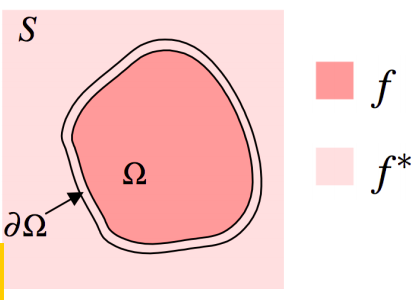
\includegraphics[width=6cm]{Image/1.png}
		\caption{Target}
		\label{Target}
	\end{minipage}
	\begin{minipage}[t]{0.48\textwidth}
		\centering
		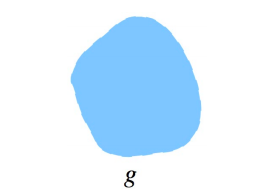
\includegraphics[width=6cm]{Image/2.png}
		\caption{Source}
		\label{Source}
	\end{minipage}
\end{figure} 
As showing in \ref{Target}, we want to embedding the \ref{Source} into the $\Omega$
place, so we need to give the $\partial \Omega$. Before that, first we should give a place mapping function from source image to the target image.
\newline
Given an assumption that the $S$ have a larger size of width and height than $g$:
\begin{itemize}
	\item[1] Discuss the simplest case, both $S$ and $g$ are rectangles, which means we only need to build the mapping relationship of the points on the 4 corners.
	\item[2] Discuss adding  $\partial \Omega$. In this case, $g$ is a 2D plane enclosed by $\partial \Omega$ and surrounded by a rectangle $G$. At this point, we need to use two parts to describe $g$, mask and basic. 
	\item[3] Regard $G$ as an image, mask is an image of the same size as $G$, and all values set to 0 or 1, 0 indicate that these pixels are not included in $g$, 1 means that it belongs to $g$. In particular, the pixels $\in \partial \Omega$ are set to 1.
\end{itemize}
\subsection{Build and solve linear system}
\subsubsection{Vector field and scalar field}
Only consider a single channel of image, we can use a function $I$, assigning the coordinate to pixel value, which is a scalar, then define a scalar field as follow:  
\begin{equation*}
\begin{aligned}
I(x,y):\ \mathcal{R}^2 \rightarrow \mathcal{R}\\
\frac{\partial I}{\partial x} = u(x,y):\mathcal{R}^2 \rightarrow \mathcal{R} \\
\frac{\partial I}{\partial y} = v(x,y):\mathcal{R}^2 \rightarrow \mathcal{R} \\
\end{aligned}
\end{equation*}
More over:
\begin{equation*}
\begin{aligned}
\text{Curl of the gradient} \nabla \times \nabla I(x,y) = \frac{\partial^2}{\partial y \partial x}I(x,y)-\frac{\partial^2}{\partial x \partial y}I(x,y) \\
\text{Divergence of the gradient}  \nabla \cdot \nabla I(x,y) = \frac{\partial^2}{\partial x^2}I(x,y)+\frac{\partial^2}{\partial y^2}I(x,y) \\
= Laplacian = \Delta I(x,y)
\end{aligned}
\end{equation*}
\subsubsection{Poisson blending}
The key idea is that when blending, retain the gradient information as best as possible, back to the format given as \ref{Target}, in which we define the source image $g$ as a integrate vector field , form the Poisson blending as integrate vector field $\nabla g$ with Dirichlet boundary conditions $f^*$
\newline
So, we need to 
\begin{equation*}
\begin{aligned}
\nabla f = \nabla g\ \text{inside}\ \Omega \\
f = f^*\ \text{at the boundary of}\ \partial \Omega \\
\min_{f} \iint_{\Omega}|\nabla f - v|^2\ \text{with}\ f|_{\partial \Omega}=f^*|_{\partial \Omega}
\end{aligned}
\end{equation*}
For the final formula,the first part would make the gradient of $f$ looks like the vector field $v$,$f$ is equivalent to $f^*$ at the boundaries, for now we induce the Poisson equation: 
\begin{equation*}
\begin{aligned}
\Delta f = div\ v\ over\ \Omega\ \text{with}\ f|_{\partial \Omega}=f^*|_{\partial \Omega} \\
\end{aligned}
\end{equation*}
For discrete images:
\begin{equation*}
\begin{aligned}
\text{For each piexl:}
(\nabla f)(x,y) = (\nabla . v)(x,y)\\
-4f_p+\sum_{q \in N_p}f_q = (u_x)_p+(v_y)_p
\end{aligned}
\end{equation*}
Equivalent to a linear system $Af = b$
\subsubsection{Solving the linear system}
Convert the system to a least-squares problem:
\begin{equation*}
\begin{aligned}
E_{LLS} = \|Af-b\|^2 = f^T(A^TA)f-2f^T(A^Tb)+\|b\|^2 \\
\frac{\partial E}{\partial f}=(A^TA)f-A^Tb\\
\end{aligned}
\end{equation*}
Where we use the conjugate gradient descent to solve this problem.
\subsection{Boundary optimization}
\subsubsection{Target of optimization}
For we want to reduce the color variance along the boundary, so the target should have
\begin{equation*}
\begin{aligned}
minE(\partial \Omega, k) = \sum_{p\in\partial\Omega}((f_t(p)-f_s(p))-k)^2 \\
s.t. \in \partial \Omega \\
f(p):(x,y)\in R^2\rightarrow(r,g,b) \in R^3
\end{aligned}
\end{equation*}
E represent the color deviation of the boundary.
\subsubsection{Iterative method}
\begin{itemize}
	\item[1] Initialize $\Omega$ as $\Omega_0$
	\item[2] Given the current boundary $\partial\Omega$
	\begin{equation*}
	\begin{aligned}
	\frac{\partial E(\partial \Omega,k)}{\partial k} = 0\\
	k = \frac{1}{|\partial \Omega|}\sum_{p\in \partial \Omega}(f_t(p)-f_s(p))
	\end{aligned}
	\end{equation*}
	$|\partial \Omega|$ is the length of the boundary, so k mean average color difference on the boundary.
	\item[3]Given the current k, we optimize the boundary $\partial \Omega$.In this part, we
	should find the shortest path which have the least with with given k.To deal with this problem, we should determine the basic element.
	\paragraph{Node} Regarded as each pixel as a node with at most 4 edge connect to the nearby pixel with 4 edges.
	\paragraph{Edge} The value of edge is compute by the distance of two nodes with the color space, form like the L2-norm. 
	\paragraph{Start} Obviously, all pixels are connected with the assumption showing before. For we want to draw a enclose $\partial \Omega$ , we using a cut C connect the $\Omega_{obj}$ and $\Omega_0$, then remove all edges crossing the cut. 
	\paragraph{End}All path should ending at the neighboring pixels on the other of cut.
	\item[4]Repeat steps 2 and 3 until the E does not decrease.
\end{itemize}

\subsubsection{Complex}
Review all steps listed before, assume we have $M$ pixels in the cutting $C$, for each $m \in M$, we need to find a best enclose $\partial \Omega_m$, finally get the globally $minE$ as the 
$\partial \Omega_{best}$.
\\
Assume we do $x_i$ iteration for $m_i \in M$, even when $m_i$ only have 1 ending target, we still need $\sum^{m \in M}_i x_i$ times finding process with the complexity $O(nlogn)$ with direct using Dijkstra.We use a simple parallel work to do this, much faster.
\section{Experiments}
\subsection{Boundary optimization}
\subsubsection{Getting the basic outline}
Using a simple gui, draw a list of points in order, than get a convex poly as the mask part.
\begin{figure}[htbp]
	\centering
	\begin{minipage}[t]{0.48\textwidth}
		\centering
		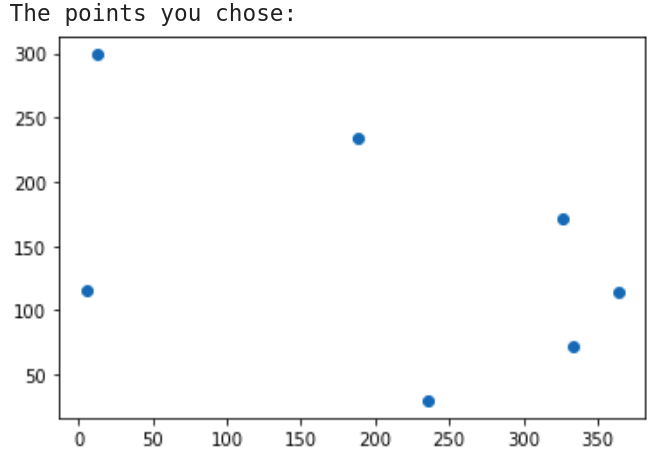
\includegraphics[width=6cm]{Image/3-1.png}
		\caption{points}
	\end{minipage}
	\begin{minipage}[t]{0.48\textwidth}
		\centering
		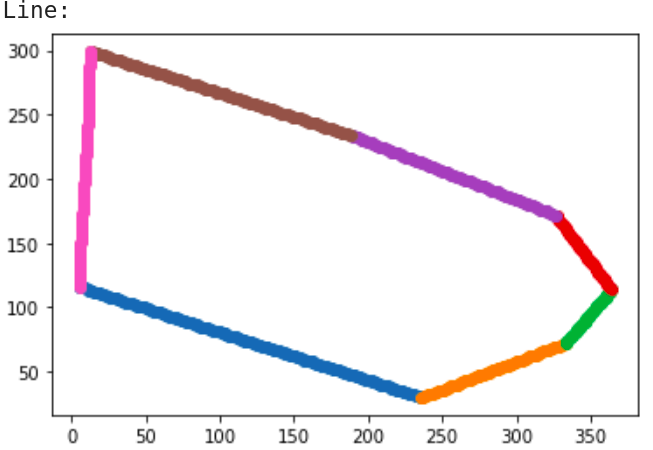
\includegraphics[width=6cm]{Image/3-2.png}
		\caption{line}
	\end{minipage}
\end{figure}
\newpage
\subsubsection{Start with K}
Do this twice, get the inline and outline, then using the E function to start with k. As in \ref{Outline}, where
the green is the object, the red part is fine to adjust, and the black was not selected part.Then the close connect between from black to green is the cut.Then as showing in \ref{cut}, the blue and white line is the two side of in this cut.
\begin{figure}[htbp]
	\centering
	\begin{minipage}[t]{0.48\textwidth}
		\centering
		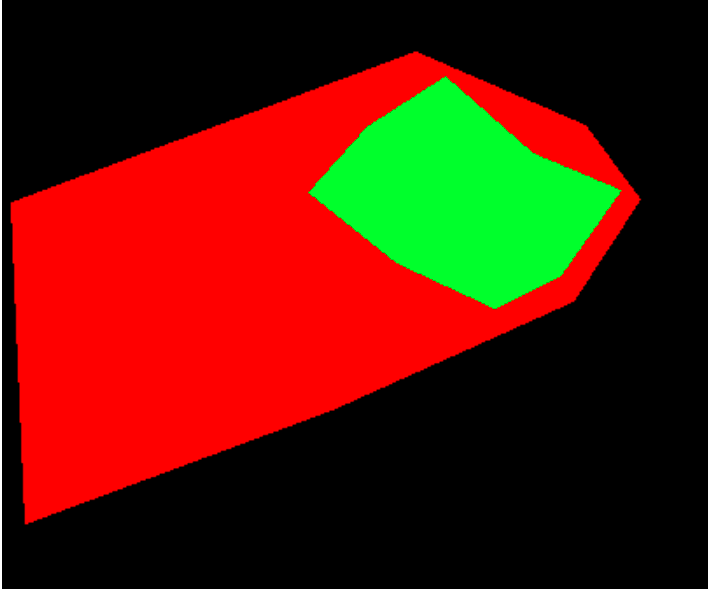
\includegraphics[width=6cm]{Image/4-1.png}
		\caption{Outline}
		\label{Outline}
	\end{minipage}
	\begin{minipage}[t]{0.48\textwidth}
		\centering
		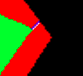
\includegraphics[width=6cm]{Image/4-2.png}
		\caption{cut}
		\label{cut}
	\end{minipage}
\end{figure}
\subsubsection{Optimization}
After this, write the information to the file as $Node$,$Edge$,$task$, using go version program to find the path as:
\begin{figure}[htbp]
	\centering
	\begin{minipage}[t]{0.48\textwidth}
		\centering
		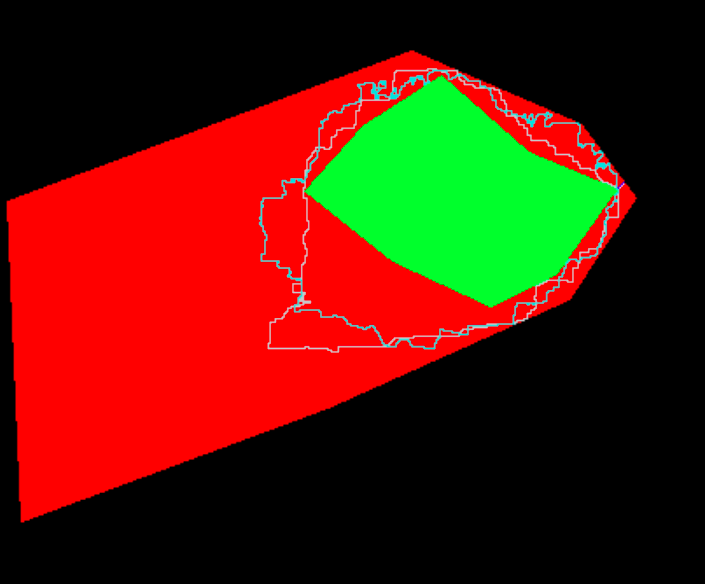
\includegraphics[width=6cm]{Image/5-2.png}
		\caption{Opt1}
	\end{minipage}
	\begin{minipage}[t]{0.48\textwidth}
		\centering
		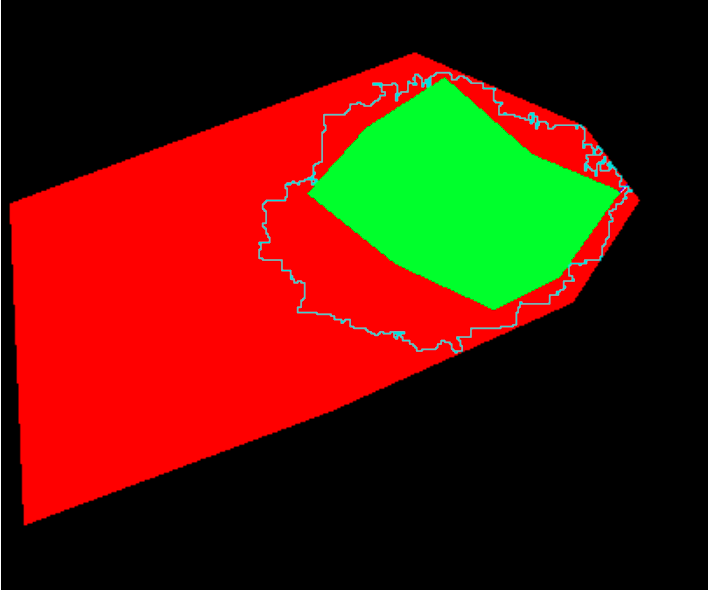
\includegraphics[width=6cm]{Image/5-1.png}
		\caption{Opt2}
	\end{minipage}
\end{figure}

\subsubsection{Get mask}
Using the best k, we get could get the mask we need, for we do not draw a good basic mask, the result is just not well, but should say that this algorithm basically converges once.
\begin{figure}[htbp]
	\centering
	\begin{minipage}[t]{0.48\textwidth}
		\centering
		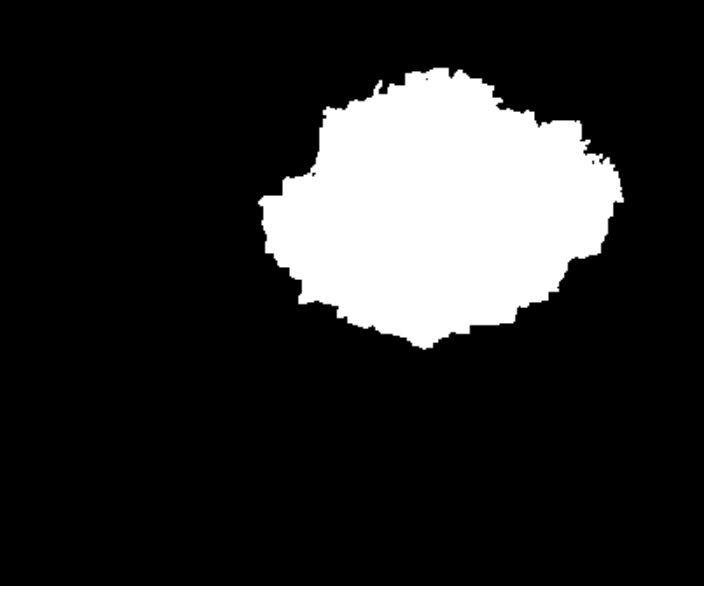
\includegraphics[width=6cm]{Image/6-1.png}
		\caption{Mask}
	\end{minipage}
	\begin{minipage}[t]{0.48\textwidth}
		\centering
		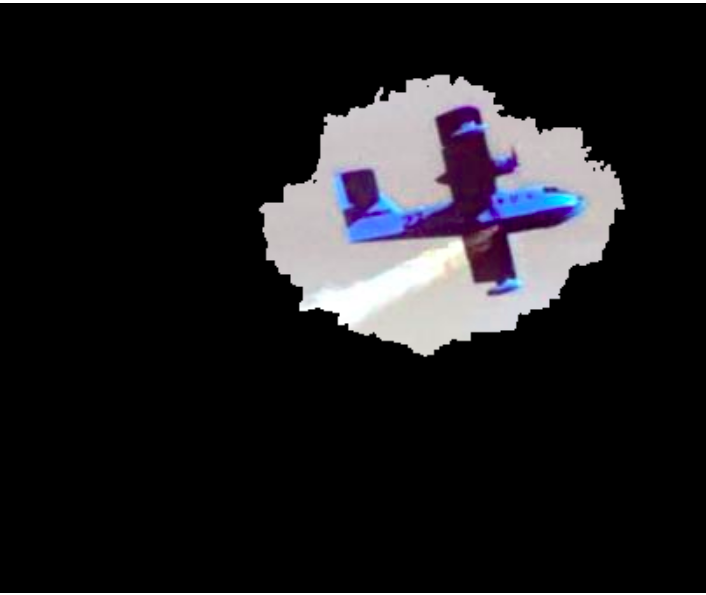
\includegraphics[width=6cm]{Image/6-2.png}
		\caption{photo}
	\end{minipage}
\end{figure}
\subsection{Blending}
\subsubsection{Form}
Only a few tricks need to talk about:
\paragraph{Matrix}
For computation, instead of build each line of the linear matrix, use $Lf = Lg$ instead of $Af=g$.
\paragraph{Solver}
$spare.linalg.cg$ is reasonable, but $spsolve$ is more quick in testing(almost $\times3$)
\begin{figure}[htbp]
	\centering
	\begin{minipage}[t]{0.48\textwidth}
		\centering
		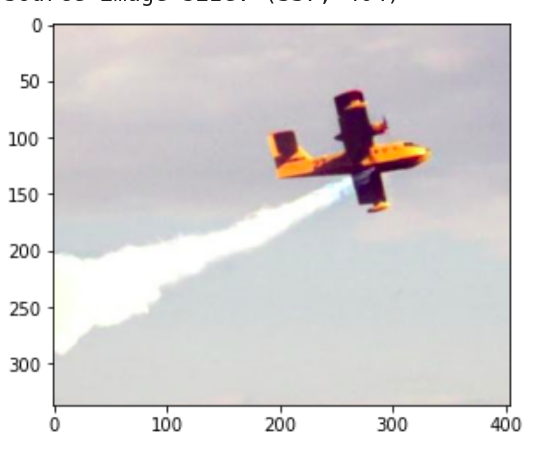
\includegraphics[width=6cm]{Image/7-1.png}
		\caption{Basic}
	\end{minipage}
	\begin{minipage}[t]{0.48\textwidth}
		\centering
		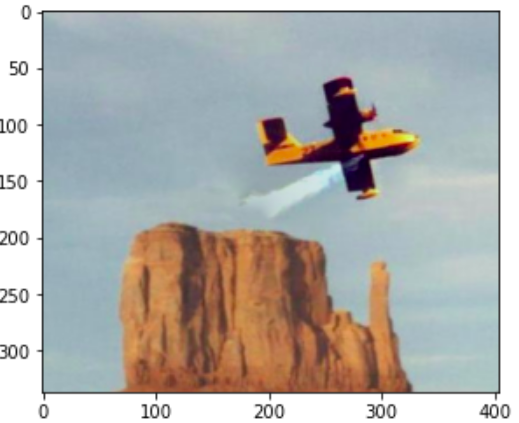
\includegraphics[width=6cm]{Image/7-2.png}
		\caption{Blending}
	\end{minipage}
\end{figure}
\section{Conclusion}

\subsection{algorithms}
There several special algorithm:
\paragraph{Draw a line}
Define at the first part of line.ipynb, Bresenham’s algorithm, achieve to draw the outline of the mask showing as before.
\paragraph{Finding the other side of a line}
To make the other side of the cut. we use the cross product to define if a point is on the target side of a line, the detail write in markdown in ipynb.
\subsection{performance}
\paragraph{Parallel}Easy to see that for each $m_i$ in cut, finding the $\partial \Omega_{m_i}$ with $minE$ is independent, using a go version code to do a multithreads work,
detail see the "path-find.md"

\section{Code}
https://github.com/fangwater/cs276lab/tree/main/assignment2



\end{document}